% !TEX options=--shell-escape
\documentclass{beamer}   	% use "amsart" instead of "article" for AMSLaTeX format
\usepackage{geometry}                		% See geometry.pdf to learn the layout options. There are lots.
%\geometry{landscape}                		% Activate for rotated page geometry
%\usepackage[parfill]{parskip}    		% Activate to begin paragraphs with an empty line rather than an indent
\usepackage{graphicx}				% Use pdf, png, jpg, or eps§ with pdflatex; use eps in DVI mode
								% TeX will automatically convert eps --> pdf in pdflatex	

\usepackage{amssymb}
\usepackage{diagbox}
\usepackage{amsmath}
\usepackage{amsthm}
\usepackage{enumerate}
\usepackage{mathrsfs}
\usepackage[utf8]{inputenc}
\usepackage{tikz}
\usepackage[outputdir=build]{minted}
\theoremstyle{definition}
\newtheorem*{defn}{Definition}
\newtheorem*{prop}{Proposition}
\newtheorem*{eg}{Example}
\newtheorem*{thm}{Theorem}
\newtheorem*{corol}{Corollary}
\newtheorem{ex}{Exercise}[section]
{\theoremstyle{plain}
\newtheorem*{rmk}{Remark}
\newtheorem*{rmks}{Remarks}
\newtheorem*{lt}{Last time}
}
\newtheorem*{lem}{Lemma}
\usepackage{color}
\usepackage{CJK}
\usepackage{tcolorbox}
\usepackage{listings}
\newcommand{\rust}[1]{\mintinline{Rust}{#1}}
\newcommand{\husky}[1]{\mintinline{Rust}{#1}}
\newcommand{\cpp}[1]{\mintinline{cpp}{#1}}
\newcommand{\highlight}[1]{\textcolor{orange}{#1}}
\newcommand{\expect}{\mathop{\mathbb{E}}}
\newcommand{\argmax}{\mathop{\text{argmax}}}
\newcommand{\argmin}{\mathop{\text{argmin}}}

\title{Towards Meaningful Deep Learning Theories}
\author{Xiyu Zhai}
\date{}							% Activate to display a given date or no date

\begin{document}
\maketitle

\begin{frame}
\frametitle{Self Introduction}
I'm a sixth year PhD student, advised by Alexander Rakhlin.

I first worked on \highlight{theories of machine learning and deep learning},
\begin{itemize}
	\item \highlight{Optimization of Ultra Wide Neural Network}.

	We proved neural networks when ultra wide can converge to global minima.

	The techniques we discovered remain one of the most prevalent in the field.
	\item \highlight{Good Generalization Despite Zero Training Loss}.

	Demystify why some ML algorithms (deep learning in particular) can interpolate the whole training set yet generalize well.

	We show that high dimensionality is the key.
\end{itemize}
\end{frame}
\begin{frame}
	
\frametitle{Self Introduction}
I'm now working on expressive power of transformers, including
\begin{itemize}
	\item transformer for vision tasks.

	Differences between transformer and CNNs.
	\item transformer for language tasks from a \highlight{programming language} perspective, such as syntax parsing, type inference checking.
\end{itemize}

Hopefully, these will shed light upon better architectures.
\end{frame}
\begin{frame}
\frametitle{Self Introduction}
Unfortunately, \highlight{huge gaps} still remain between theory and practice, even to this day.

I've been working on a new project for the last three years for next generation AI methods, it consists of 
\begin{itemize}
	\item machine learning theory \highlight{beyond function approximation}
	\item \highlight{a new programming language} called husky for next generation AI and software.

	It's a lot of work. (120k lines of source code in Rust)
	\item new machine learning algorithms that \highlight{only be implemented in the new language}
\end{itemize}

It's work in progress. Needs several months before the first results.

Will be covered briefly today. Maybe more in PhD defense.
\end{frame}
\begin{frame}
\frametitle{Talk Today}
I shall talk about
\begin{itemize}
	\item our theoretical work on optimization theory of ultra wide neural networks.
	\item our theoretical work on interpolation yet generation phenomenon.
	\item ongoing work on transformer expressive power for CV/NLP
	\item why the gap between theory and practice is so huge.
	\item theories of machine learning theory beyond generalization briefly.
	\item the new programming language for AI briefly.
\end{itemize}
\end{frame}

\begin{frame}
\frametitle{Machine Learning Theory: PAC Learning}

PAC is short for Probably Approximately Correct.

$\mathcal{X}$ input space.

$\mathcal{Y}$ label/target space.

$\mathcal{C}\subseteq \mathcal{Y}^\mathcal{X}$ concept class.

$\mathcal{H}\subseteq \mathcal{Y}^\mathcal{X}$ hypothesis class.

$S=(\mathcal{X}\times \mathcal{Y})^m$ dataset space.

$\rust{loss}\in \mathcal{Y}^\mathcal{Y}$ is loss.

\begin{defn}[PAC-learning]
A concept class $\mathcal{C}$ is said to be PAC-learnable if there exists an algorithm $\mathcal{A}$ mapping from $S$ to $\mathcal{H}$ such that for any $c\in \mathcal{C}$ and any distribution $\mathcal{D}$ on $\mathcal{X}\times\mathcal{Y}$ satisfying $y=c(x)$, with high probability
\begin{equation}
	\expect\limits_{(x,y)\sim \mathcal{D}}\expect\limits_{S\sim \mathcal{D}^m}\rust{loss}(A(S)(x),y)
\end{equation}
is small for $m$ large enough.
\end{defn}

\end{frame}

\begin{frame}
	Two fundamental problems arises
	\begin{itemize}
		\item Optimization.

		When $\mathcal{A}$ is taken to be an optimization process that minimizes training loss, can global minima be achieved?

		Not true in general, can be NP-hard.
		\item Generalization.

		The difference between testing error and training error.
	\end{itemize}

	Deep learning blows away traditional understanding in both aspects.

	Our theories can explain them to some extend.
\end{frame}

\begin{frame}
\frametitle{Year 1992: optimization theory of deep learning be like}
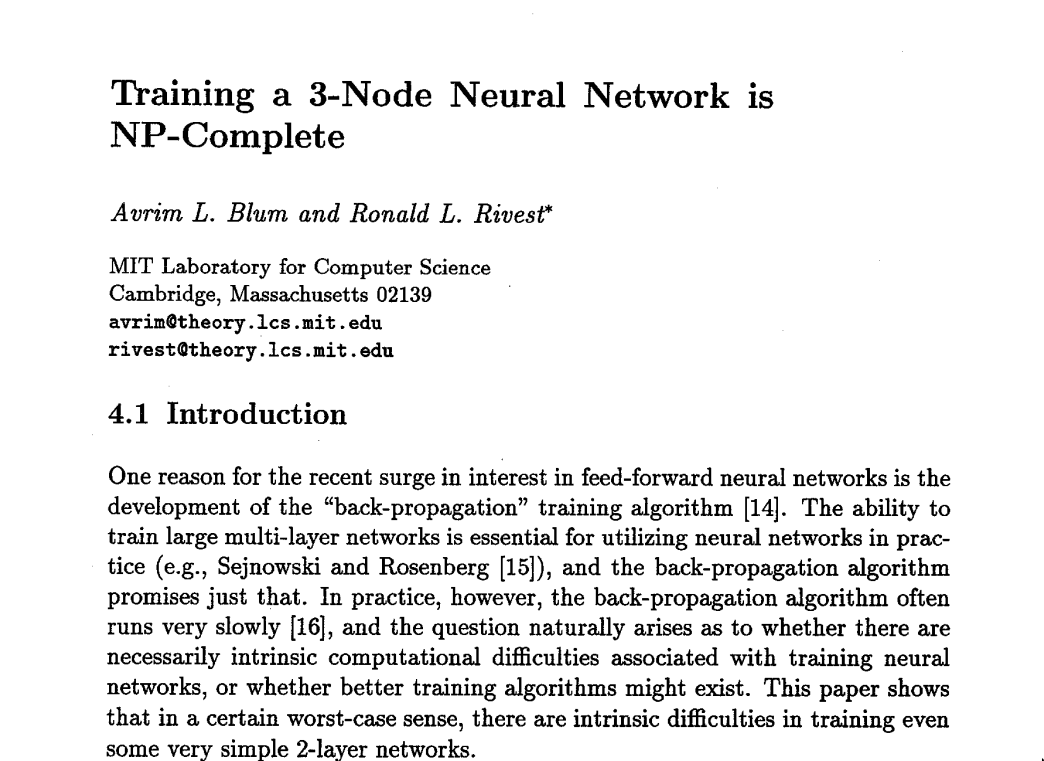
\includegraphics[width=\linewidth]{train_nn_is_np_complete.png}
\end{frame}

\begin{frame}
\frametitle{Today: optimization of neural networks is not intractable}
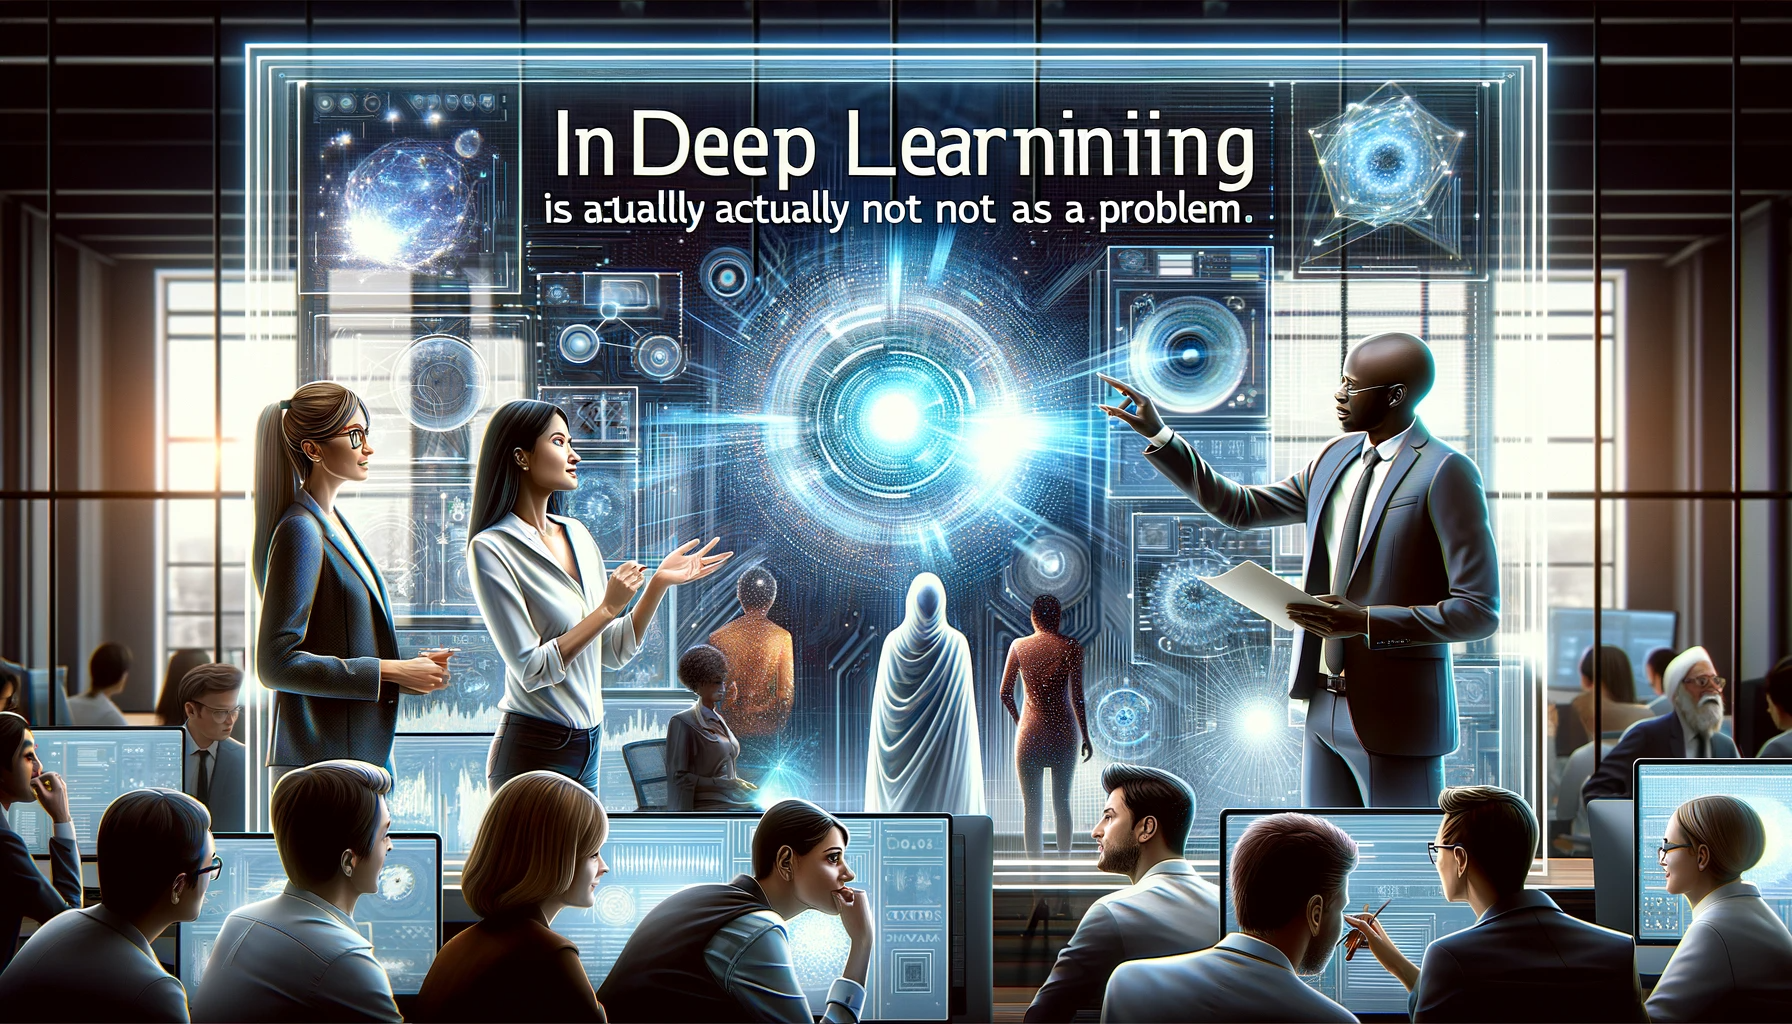
\includegraphics[width=\linewidth]{nn_is_not_a_problem.png}
\end{frame}

\begin{frame}
In \cite{latexcompanion}, experiments show that neural networks can fit random labels.

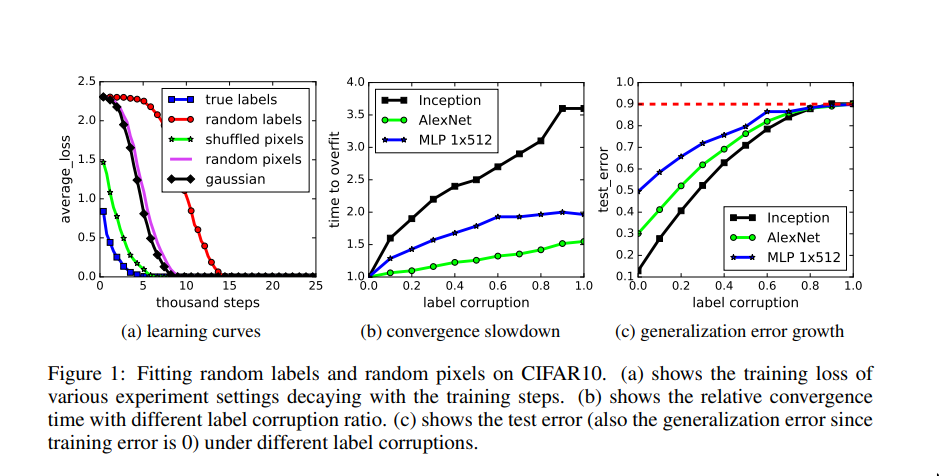
\includegraphics[width=\linewidth]{overfit_random_noise.png}

\begin{thebibliography}{9}
\scriptsize
\bibitem{latexcompanion} 
Chiyuan Zhang* and Samy Bengio and Moritz Hardt and Benjamin Recht and Oriol Vinyals
\textit{Understanding Deep Learning Requires Rethinking Generalization}.
\end{thebibliography}
\end{frame}

\begin{frame}[t]
\frametitle{Overparametrization might be the key}

Overparametrization refers to number of model parameters being much larger than

For CIFAR10 with 50k samples,

\begin{table}[h]
\centering
\begin{tabular}{|l|c|}
\hline
\textbf{Model} & \textbf{Number of Parameters} \\
\hline
Inception & 1.6M \\
Alexnet & 1.4M \\
MP 1x512 & 1.2M\\
\hline
\end{tabular}
% \caption{Number of parameters for various neural network models on CIFAR-10}
\label{tab:my_label}
\end{table}

For ImageNet with 1.2M number of samples,
\begin{table}[h]
\centering
\begin{tabular}{|l|c|}
\hline
\textbf{Model} & \textbf{Number of Parameters} \\
\hline
Inception & 43M \\
Alexnet & 61M \\
Resnet-152 & 60M\\
VGG-19 & 143M\\
AmoebaNet & 600M\\
\hline
\end{tabular}
\end{table}
\end{frame}

\begin{frame}
\frametitle{We Prove Overparameterization Helps Optimization}
\begin{thm}
	[informal version, \cite{op1}, \cite{op2}]
	If width $\ge$ poly(n) and proper random initialization, gradient descent on over-parameterized neural networks (one-layer or multi-layer) converges to global optimum with \highlight{0 optimization error}.
\end{thm}

\begin{proof}
	[Sketch of Proof]

	For ultra wide neural networks with proper initialization, we prove using random matrix techniques the dynamics will remain inside a \highlight{good regime}
\end{proof}

* means equal contributions.

\begin{thebibliography}{9}
\scriptsize
\bibitem{op1}
Simon S. Du* and Jason D. Lee* and Haochuan Li* and Liwei Wang* and Xiyu Zhai*
Gradient Descent Provably Optimizes Over-Parameterized Neural Networks
\bibitem{op2} 
Simon S. Du* and Xiyu Zhai* and Barnabas Poczos and Aarti Singh
Gradient Descent Finds Global Minima of Deep Neural Networks
\end{thebibliography}
\end{frame}

\begin{frame}
The optimization loss landscape be like
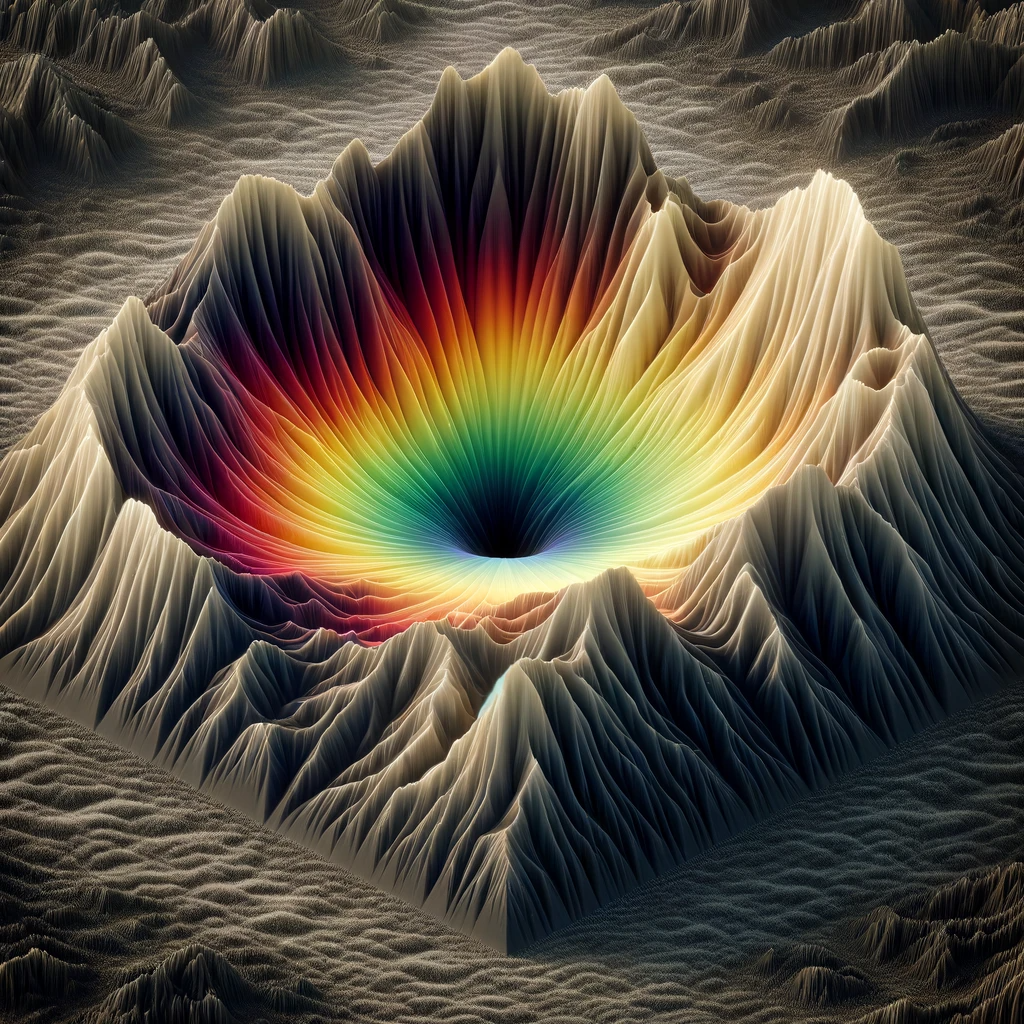
\includegraphics[width=\linewidth]{ultra_wide_nn_landscape.png}
\end{frame}

\begin{frame}
Let $\Omega$ be the good regime, we proved that
\begin{itemize}
	\item if the weight lies in $\Omega$, the training dynamics is approximately linear.

	The kernel is exactly Neural Tangent Kernel in \cite{ntk}.
	\item If the training dynamics is approximately linear, it will not leave $\Omega$
\end{itemize}

We proved that initialization is within $\Omega$, then using induction on continuous time, we proved the weight $\Omega$ during the whole training process and 
\begin{thebibliography}{9}
\scriptsize
\bibitem{ntk}
	Neural Tangent Kernel: Convergence and Generalization in Neural Networks
\end{thebibliography}
\end{frame}

\begin{frame}
\frametitle{Strengths}
The strengths of this line of work are
\begin{itemize}
	\item math is elegant and simple with clear insight as compared with \cite{yzl}.

	It's so simple that it surprises me that no one've done it before.
	\item connects with kernel methods in traditional machine learning and statistical learning.

	It's a bridge 
\end{itemize}

They're the reasons many results are built upon our results in the passing years.
\begin{thebibliography}{9}
\scriptsize
\bibitem{yzl} 
Zeyuan Allen-Zhu* and Yuanzhi Li* and Zhao Song*
A convergence theory for deep learning via over-parameterization
\end{thebibliography}
\end{frame}

\begin{frame}
\frametitle{Limitations}
The fundamental limitations of our work are
\begin{itemize}
	\item overparametrization is unrealistic in practice.

	For one thing, inference efficiency matters, it's more desirable to have fewer parameters.
	\item the actual dynamics might work under different mechanisms.
\end{itemize}

\vspace{5mm}

\vspace{5mm}

Mystery is not entirely resolved.

Keep calm and carry on!
\end{frame}

\begin{frame}
\frametitle{Generalization}
Traditional thinking: tradeoff between training error and generalization

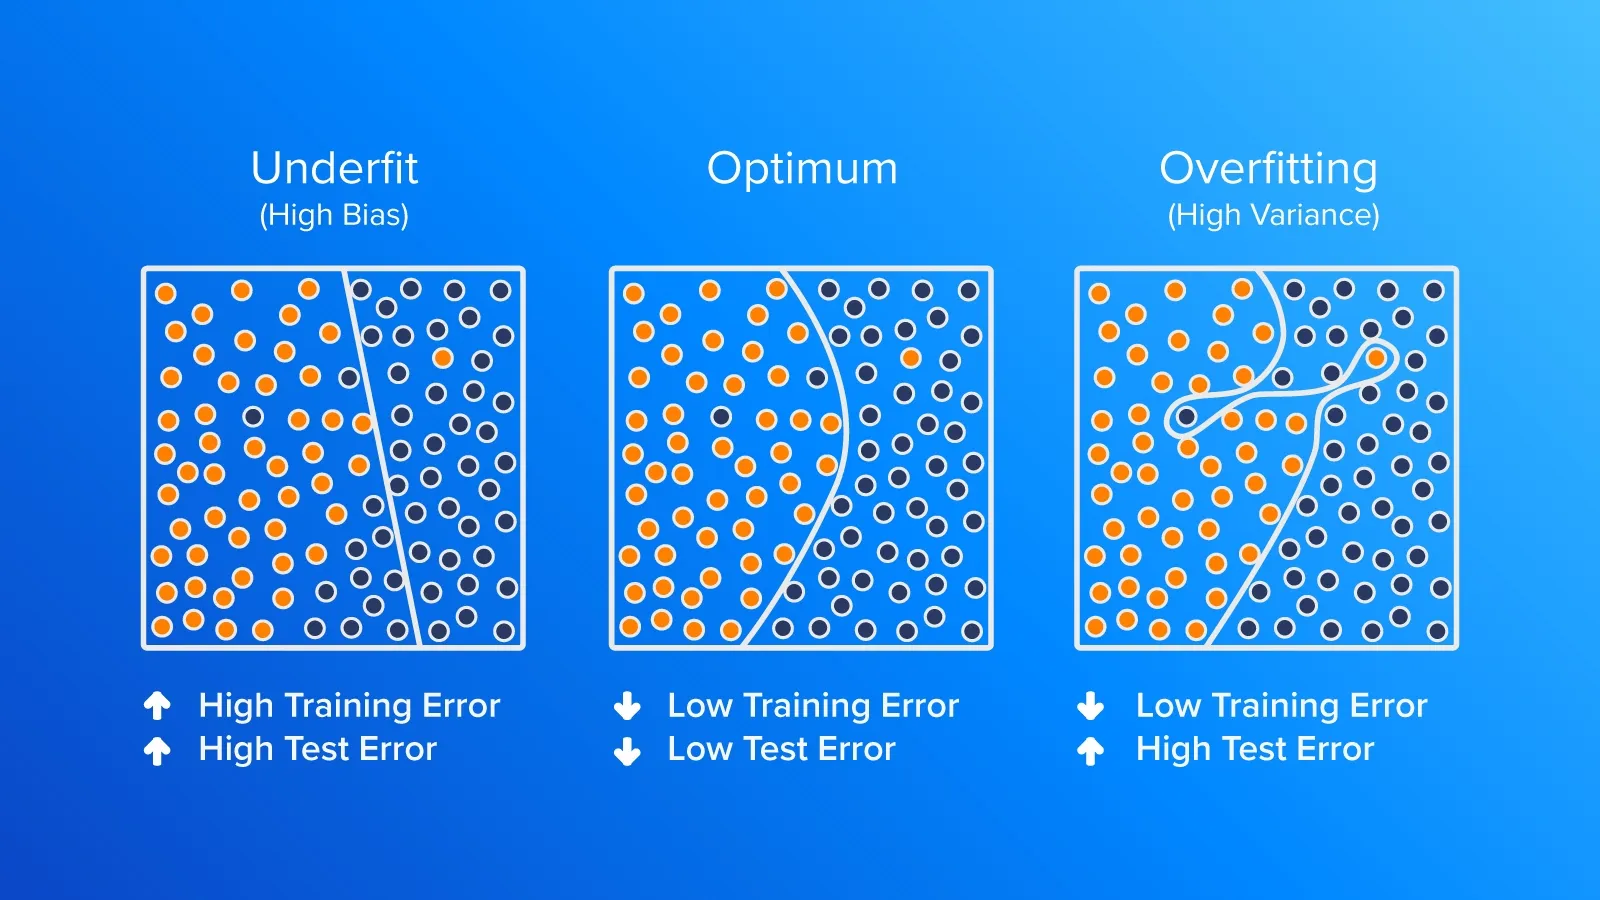
\includegraphics[width=\linewidth]{fit}
\end{frame}

\begin{frame}{Generalization}
Expectation...
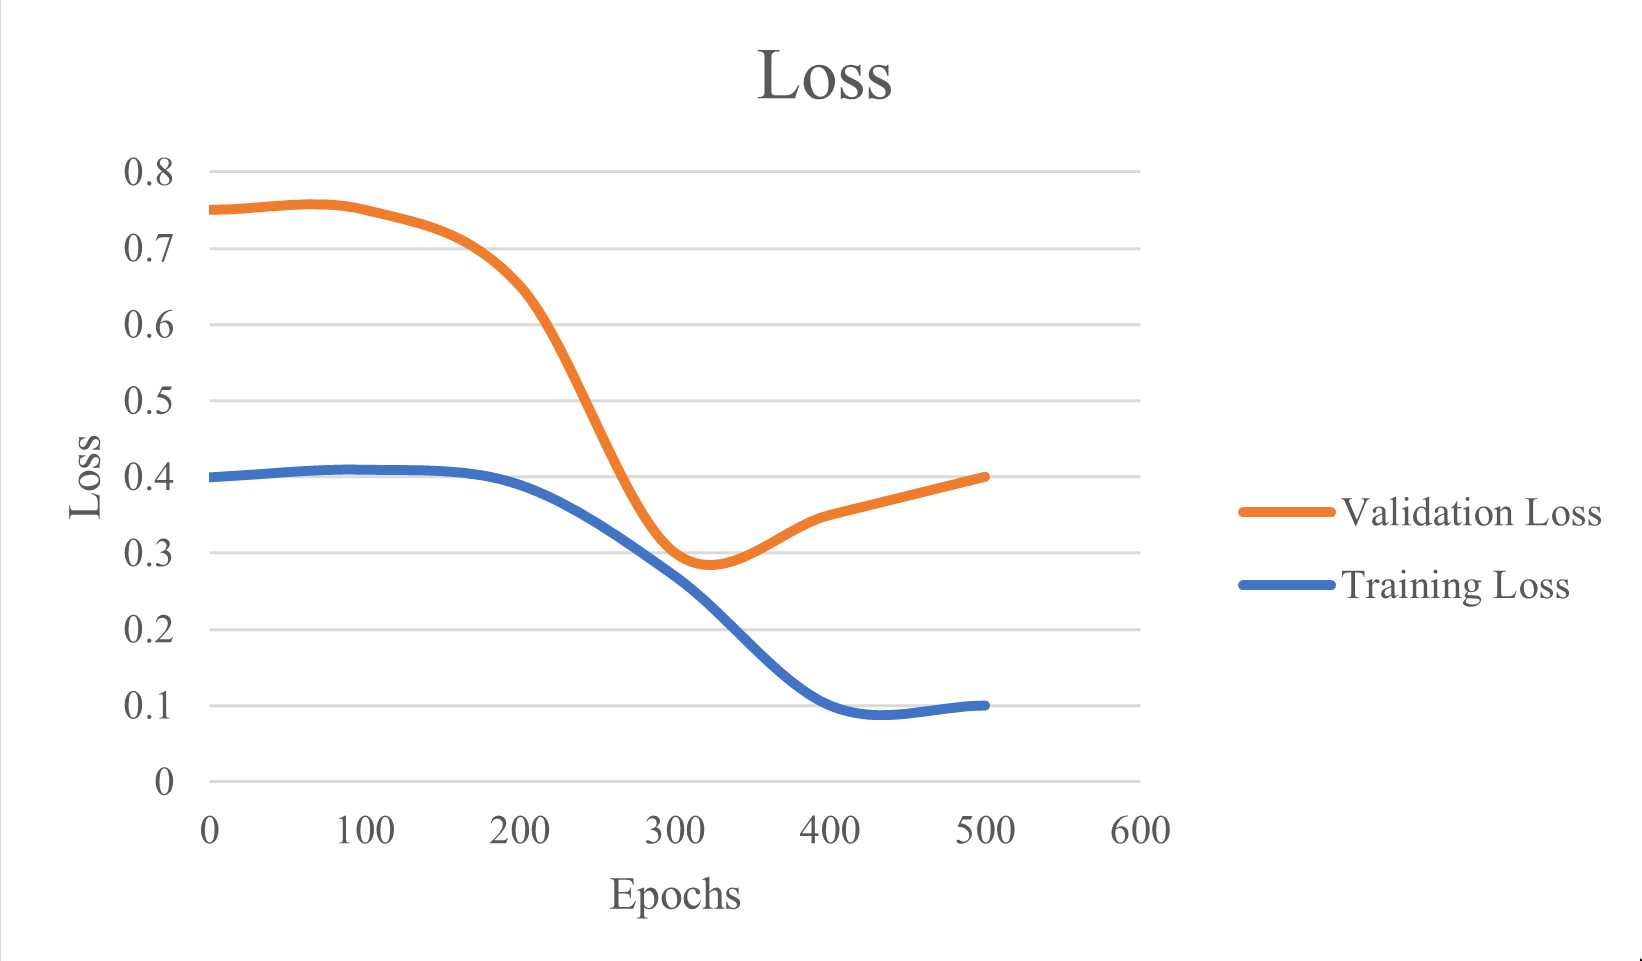
\includegraphics[width=\linewidth]{loss_curve_expected.png}
\end{frame}

\begin{frame}{Generalization}
Reality can be ...
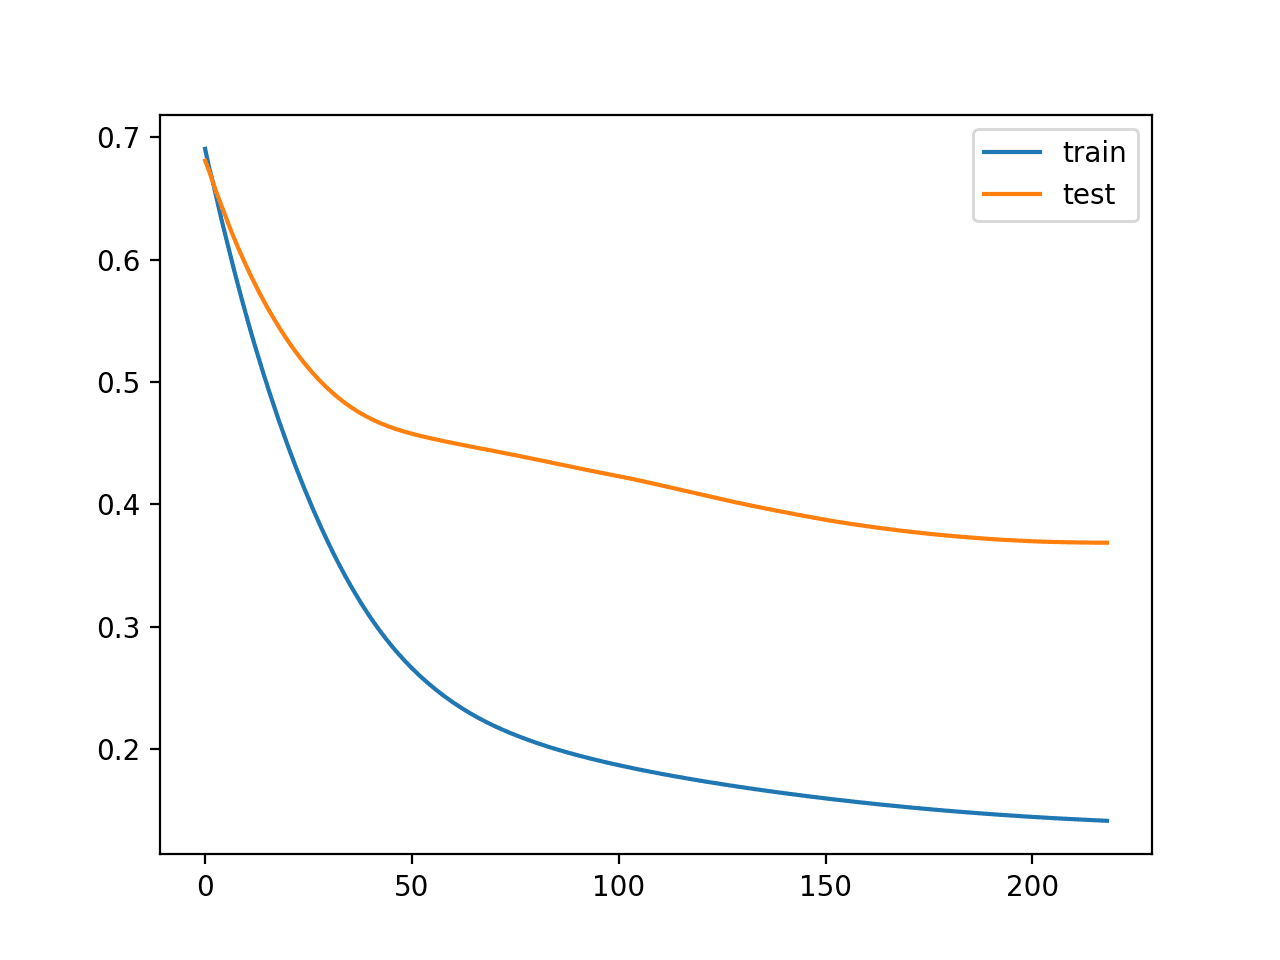
\includegraphics[width=\linewidth]{loss_curve}
\end{frame}

\begin{frame}
\frametitle{Kernel Ridge Regression}
To focus, we choose to study kernel ridge regression for this phenomenon.

\begin{equation}
	\hat{f}\in\argmin\limits_{f\in \mathcal{H}} \frac{1}{n}\sum\limits_{i=1}^n(f(x_i)-y_i)^2+ \lambda \|f\|_\mathcal{H}^2
\end{equation}

Here $\mathcal{H}$ is a Reproducing Kernel Hilbert Space (RKHS) corresponding to a kernel $K$, $\|\cdot\|_\mathcal{H}$ is the corresponding RKHS norm, and $(x_1,y_1),\cdots,(x_n,y_n)\in \mathbb{R}^d\times \mathbb{R}$ are the training data.

The method interpolates the data when $\lambda = 0$, .e.
\begin{equation}
	\hat{f}(x_i)=y_i
\end{equation}

Previous work shows it performs ``unreasonably well'' in this regime.

\end{frame}

\begin{frame}
\frametitle{Previous Work}
In \cite{jint}, they studied the high-dimension regime $n\asymp d$, explicating a phenomenon of implicit regularization, due to the curvature of the kernel function, high dimensionality and favorable geometric properties of the training data, ..

High dimensionality $d$ of the input space is critical for the implicit regularization.

Question: what if dimensionality is low?

Our experiments: interpolation doesn't work for low-dimensionality.

Our theory: interpolation doesn't work for low-dimensionality.

\begin{thebibliography}{9}
\scriptsize
\bibitem{jint}
Tengyuan Liang and Alexander Rakhlin. Just interpolate: Kernel” ridgeless” regression can generalize
\end{thebibliography}
\end{frame}

\begin{frame}
	Let $f^*$ be an unknown smooth function over $\Omega=\overline{B_{\mathbb{R}^d}(0,1)}$ that is not identically zero, and $\mathcal{P}$ an unknown distribution over $\Omega$ with probability density function $\rho$ bounded as
	\begin{equation}
		0< c_ \rho\le \rho\le C_ \rho.
	\end{equation}

	Suppose $X_1,\cdots,X_n$ are sampled i.i.d according to $\mathcal{P}$, and
	\begin{equation}
		Y_i=f^*(X_i)+\xi_i
	\end{equation}
	with $\xi_i$ i.i.d. noise, let $\mathcal{S}$ denote $\{(X_i,Y_i)\}_{i=1}^n$

	\begin{thm}[\cite{cint}]
		Let $\hat{f}_c$ be the minimum-norm soultion interpolating $(x_i,y_i)$ w.r.t Laplace kernel $K_c(x,y)= c^d e^{-c\|x-y\|}$. For fixed $n$ and odd dimension $d$, with probability at least $1-O(\frac{1}{\sqrt{n}})$ over the draw of $S$,
		\begin{equation}
			\forall c> 0,\mathop{\mathbb{E}}\limits_{X\sim \mathcal{P}}\left(
			\hat{f}_c(X)-f^*(X)\right)^2\ge \Omega_d(1)
		\end{equation}
	\end{thm}
\begin{thebibliography}{9}
\scriptsize
\bibitem{cint}

Alexander Rakhlin, Xiyu Zhai. Consistency of Interpolation with Laplace Kernels is a High-Dimensional Phenomenon
\end{thebibliography}
\end{frame}

\begin{frame}
\frametitle{Intuition: Either Too Smooth Or Too Close to Zero}
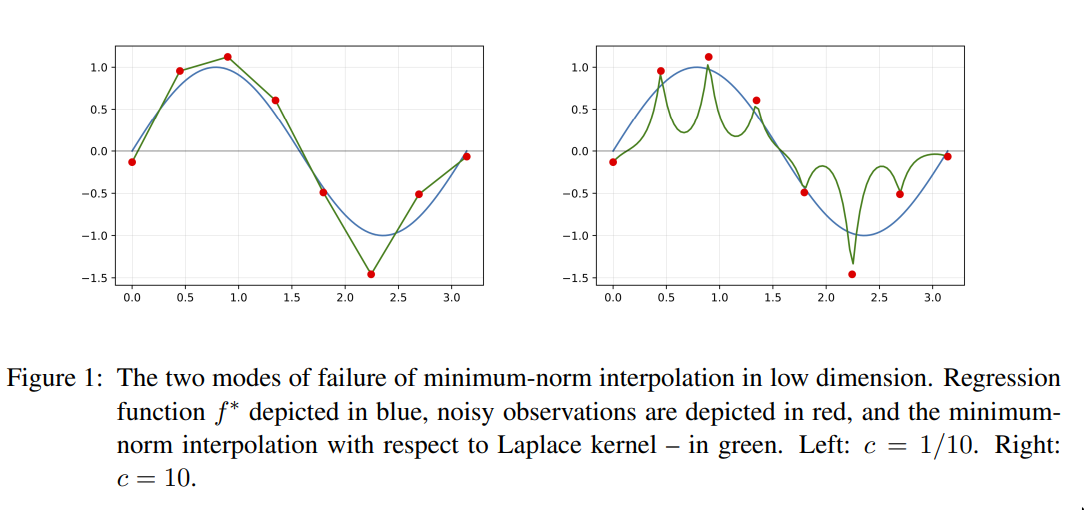
\includegraphics[width=\linewidth]{int_intuition.png}
Sketch of Proof
\begin{itemize}
	\item For hyperparameter $c$ not large, prove $\hat{f}$ is too smooth.
	\item For hyperparameter $c$ not small, prove $\hat{f}$ is too close to $0$.
	\item The two regimes overlaps and cover all possible choices of $c$.
\end{itemize}
\end{frame}

\begin{frame}
\frametitle{Connection to Deep Learning via Neural Tangent Kernel}

The conclusion carries over to ultra wide neural networks through our previous results.
\begin{center}
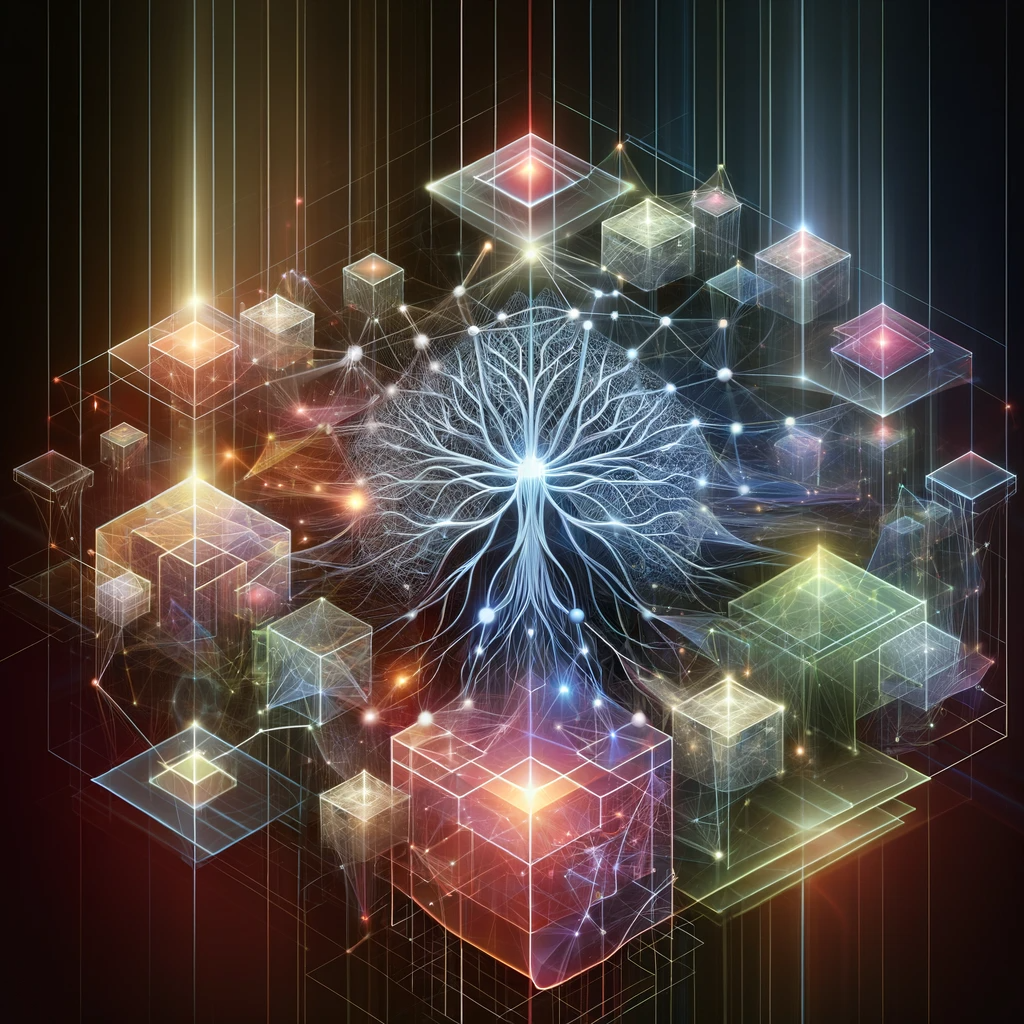
\includegraphics[width=0.9\linewidth]{ntk.png}
\end{center}
\end{frame}

\begin{frame}
\frametitle{Ongoing Work: Transformer Expressive Power for Vision Tasks}
Vision Transformer has 24 layers as agains ResNet hundreds of layers. How could it work?
\begin{itemize}
	\item linear convolution with arbitrary window size
	\item template matching
	\item congregation of small patterns
\end{itemize}
\frametitle{Ongoing Work: Transformer Expressive Power for Natural Language Processing Tasks}
\end{frame}

\begin{frame}
Natural language is not programming language, but similar.

Type theory of programming language can be used to explain comparative illusion, for example why the following sentence is not valid,


	\textcolor{blue}{`More people have been to Russia than I have'}.

As more and more people use chatgpt for writing code, transformer for programming language is meaningful for its own sake.

We shall study the theoretical computational power of transformers for
\begin{itemize}
	\item syntax parsing
	\item semantic understanding like type checking, type inference, evaluation of expression, etc
	\item code generation under constraints
\end{itemize}
\end{frame}

\begin{frame}
\frametitle{The Predicament of Deep Learning Theory}
What makes a good applied theory:
\begin{itemize}
	\item predicts experiments rather than explaining them;
	\item insights can be more important than rigor of proof;
	\item assumptions should be simple but not far from reality;
\end{itemize}

We have yet to see such wonderful things in deep learning theory.
\end{frame}

\begin{frame}
\frametitle{But Physicists Did That!}
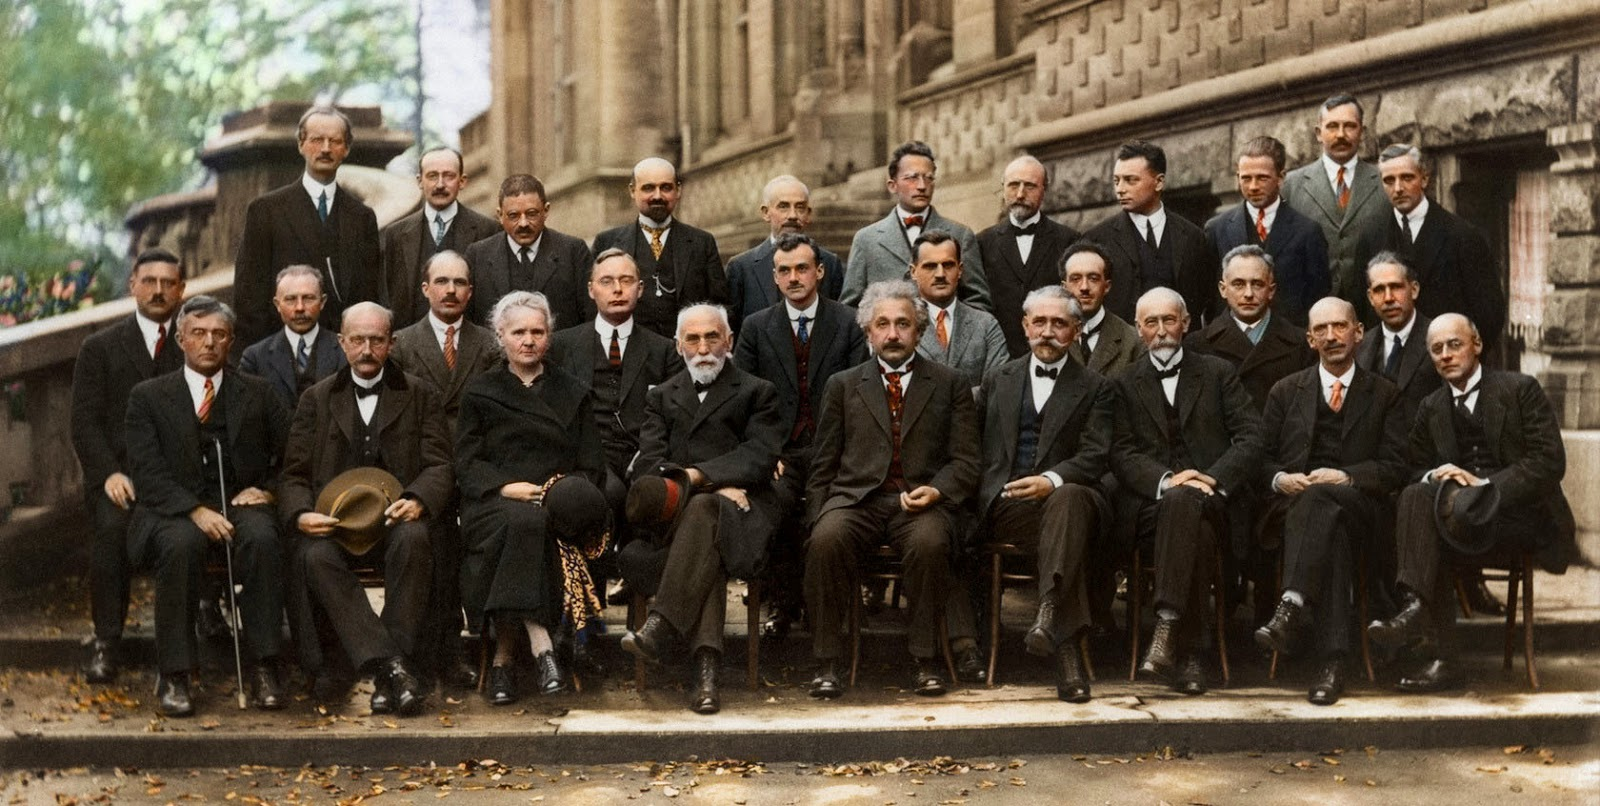
\includegraphics[width=\linewidth]{physicists.jpg}

Can we have the equivalence for deep learning theory in this century?
\end{frame}

\begin{frame}
\frametitle{Machine Learning vs Physics}

As we are at least smart as people in the last century, the problem lie in the field itself.

\begin{table}[h]
\centering
\begin{tabular}{|>{\centering\arraybackslash}m{0.3\linewidth}|>{\centering\arraybackslash}m{0.3\linewidth}|>{\centering\arraybackslash}m{0.3\linewidth}|}
\hline
 & \textbf{AI} & \textbf{Physics} \\ 
\hline
System Complexity & high & low \\
\hline
Scaling & \(10^8\) & \(10^{23}\) \\
\hline
well definedness & inverse problem, partial information, noisy & well-defined \\
\hline
experimental style & end-to-end & modular and domain specific \\
\hline
abstraction level & computation and mathematics & just mathematics \\
\hline
history & ~50yrs & thousands of years \\
\hline
history of success & a decade & hundreds of years \\
\hline
\end{tabular}
\caption{Comparison between Machine Learning and Physics}
\label{table:comparison}
\end{table}
\end{frame}

\begin{frame}
\frametitle{Is This the End of Theories?}
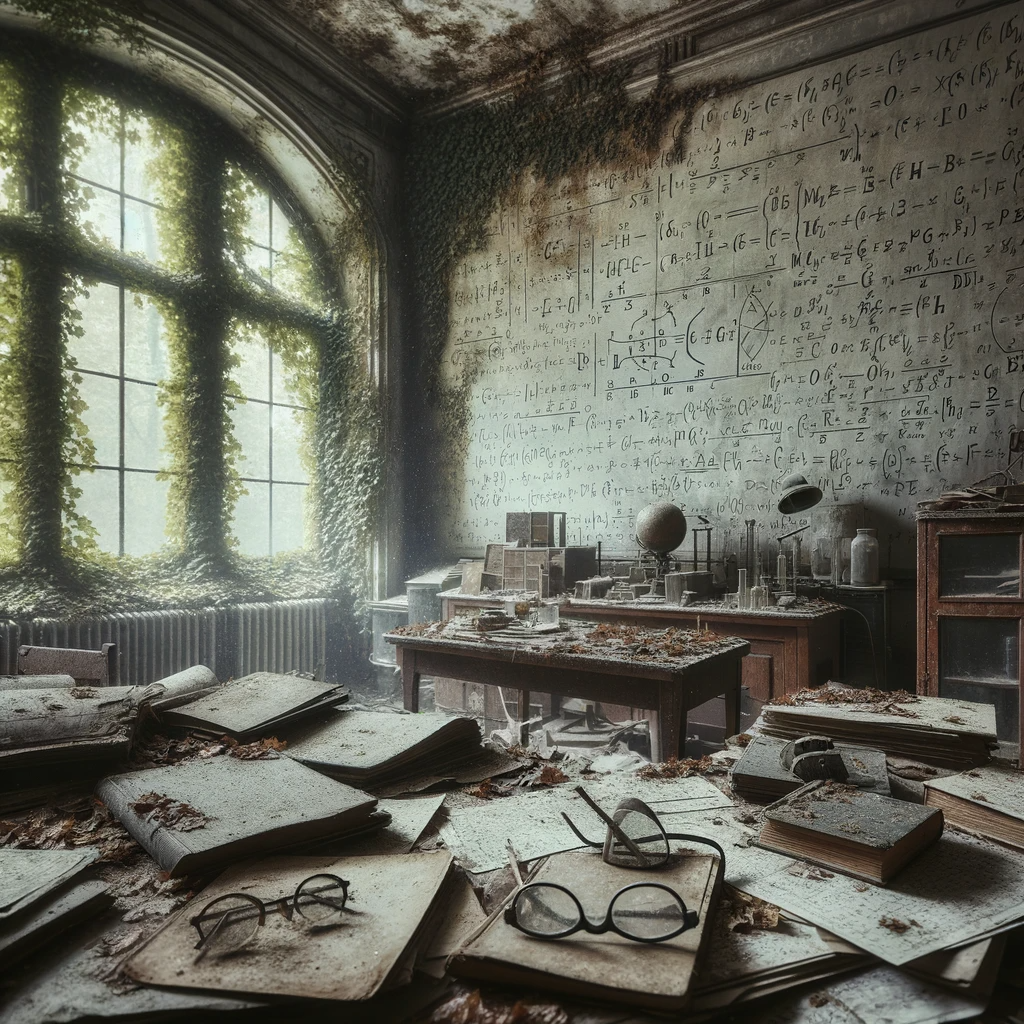
\includegraphics[width=\linewidth]{forgotten_theories.png}
\end{frame}

\begin{frame}
Personal opinion: no.

Deep learning still has serious flaws:
\begin{itemize}
	\item needs tons of data
	\item training is tricky and slow
	\item inference is slow
	\item accuracy for corner cases are not that good
\end{itemize}

Breakthroughs in theories could lead to much better AIs.
\end{frame}

\begin{frame}
\frametitle{My Theories of Next-Generation AI (sketch)}

Warning: work in progress. Several months away from prototype.

Reinvent PAC-learning.

Let's review PAC-learning.
\end{frame}

\begin{frame}
\frametitle{Review of PAC-learning}
$\mathcal{X}$ input space.

$\mathcal{Y}$ label/target space.

$\mathcal{C}\subseteq \mathcal{Y}^\mathcal{X}$ concept class.

$\mathcal{H}\subseteq \mathcal{Y}^\mathcal{X}$ hypothesis class.

$S=(\mathcal{X}\times \mathcal{Y})^m$ dataset space.

$\rust{loss}\in \mathcal{Y}^\mathcal{Y}$ is loss.

\begin{defn}[PAC-learning]
A concept class $\mathcal{C}$ is said to be PAC-learnable if there exists an algorithm $\mathcal{A}$ mapping from $S$ to $\mathcal{H}$ such that for any $c\in \mathcal{C}$ and any distribution $\mathcal{D}$ on $\mathcal{X}\times\mathcal{Y}$ satisfying $y=c(x)$, with high probability
\begin{equation}
	\expect\limits_{(x,y)\sim \mathcal{D}}\expect\limits_{S\sim \mathcal{D}^m}\rust{loss}(A(S)(x),y)
\end{equation}
is small for $m$ large enough.
\end{defn}
\end{frame}

\begin{frame}
What's missing in the picture?

\mbox{}

Everything is mathematical, there is no mention of inference computation.

\mbox{}

But actually inference computation matters, sometimes even more than training time.

Just like app development, an app is developed only once, but can be used millions of times.
\end{frame}

\begin{frame}
Examples
\begin{itemize}
	\item image/video AI generation is slow
	\item LLM is slow
	\item traditional AI methods, especially those in computer vision, often scales poorly in terms of inference efficiency, thus don't perform as well as deep learning
	\item people are using deep learning to replace slow traditional theory-based methods in solving PDE, molecules, computer graphics etcs.

	There is nothing intrinsically unknown like in statistics, but deep learning gives us a short path computationally.
\end{itemize}

As AI becomes more and more powerful, inference process of AI seems more and more computationally nontrivial.
\end{frame}

\begin{frame}
\frametitle{Hypothesis Class Can be Hard Computationally}

There could be a much smaller hypothesis $\mathcal{H}_0$ containing the ground truth, but the functions in $\mathcal{H}_0$ can be hard to compute.

So there could be another class $\mathcal{H}_1$, like neural networks that approximately contains $\mathcal{H}_0$, and the functions in $\mathcal{H}_1$ are straightforward to compute.

$\mathcal{H}_1$ is statistically more complicated, but is more feasible to learn.

\definecolor{lightblue}{rgb}{0.53, 0.81, 0.98}
\begin{center}
\begin{tikzpicture}
    \fill[lightblue] (0.5,0) ellipse (2.3cm and 2.0cm);
    \fill[yellow] (0,0) circle [radius=0.7cm];
     \node[align=center] at (0,0) {$\mathcal{H}_0$};
     \node[align=center] at (2.25,0) {$\mathcal{H}_1$};
\end{tikzpicture}
\end{center}
\end{frame}

\begin{frame}
\frametitle{Nondeterministic PAC: inference as NP problem}
Hypothesis: the inference process of many machine learning problems can be formulated more succinctly in NP form, with verifier to be learned.

More specifically, let $\mathcal{X}, \mathcal{Y}$ be input and label spaces, $W$ be parameter space, and let $\Gamma$ be a certificate space, fix $f$ a function from $\mathcal{X}\times \mathcal{Y}\times \Gamma\times W$ to $\mathbb{R}$, then we can define a hypothesis space like
\begin{equation}
	\mathcal{H}_f=\{h_w: w\in W\}
\end{equation}
where
\begin{equation}
	h_w(x,y)=\sup_{\gamma\in \Gamma} f(x,y,\gamma;w)
\end{equation}
gives the energy(or log-likelihood) of $x$ maps to $y$.

\mbox{}

Remarks: this hypothesis introduces nontrivial computational element to inference, making the problem more challenging.
\end{frame}

\begin{frame}
Most of pattern recognition in AI satisfies this, for example:
\begin{itemize}
	\item templating matching in computer vision.

	A template is a family of images indexed by say $\Gamma$, one must select $\gamma\in \Gamma$ such that the input matches the template.
	\item NLP.

	Grammar rules are verification rules.

	The meanings a word could possibly have are verification rules.

	Checking a statement makes sense is also verification.

	In RLHF,The reward model is kind of like a verifier.
	\item Robotics, world model
	\item Image Generation, GAN.

	Whether an image looks realistic is a verification process.

	So is checking whether an image satisfies the text prompt.
	\item AI for code generation/math

	External tools like Lean4, python interpreter can be used as verifier.
\end{itemize}
\end{frame}

\begin{frame}
NP-ML hypothesis explains:
\begin{itemize}
	\item many traditional AI methods are slow than deep learning.

	Deep learning is learning the solver directly.
	\item deep learning requires more data.
	\item deep learning have trouble in corner cases 
	\item humans learning are better than deep learning in many aspects
\end{itemize}
\end{frame}

\begin{frame}
\frametitle{Select-Verify Architecture}

Here we propose select-verify architecture,
\begin{center}
\begin{tikzpicture}
    % Define style for the boxes and circle
    \tikzstyle{box} = [rectangle, minimum width=2cm, minimum height=1cm, text centered, draw=black]
    \tikzstyle{circ} = [circle, minimum size=2cm, text centered, draw=black]
    
    % Draw the boxes
    \foreach \i in {1,...,3} {
        \node[box] (selector\i) at (0,-1.2*\i) {Selector \i};
    }
    
    % Draw the circle
    \node[circ] (verifier) at (4.5,-2.4) {Verifier};

    % Draw arrows from each box to the circle
    \foreach \i in {1,...,3} {
        \draw[-latex] (selector\i) -- (verifier);
    }

    % Draw an outgoing arrow from the circle
    \draw[-latex] (verifier) -- +(3.5,0);
\end{tikzpicture}
\end{center}

Selectors and verifier can be neural networks, or mixed things.

In essence, this is somehow similar to MOE (mixture of expert) +COT (chain of thought).

\end{frame}

\begin{frame}
Advantages
\begin{itemize}
	\item labels are only needed for learning the verifier.
	\item there can be a cascade of selectors, fast ones that cover common cases, slow ones that deals with border cases.

	Neural network acceleration techniques (pruning, quantization, etc.) can be used more aggressively on the selector
	\item verifier is clean, can be analyzed theoretically in a more thorough way or being totally explainable.

	Solver, on the other hand, can be arbitrarily messy.
	\item verifier can be highly modular.

	For example, imagenet has 1000 classes. Each class can have a dedicated verifier.

	The vision system can run like
	\begin{itemize}
		\item A cheap model that predicts top 10 possible classes.
		\item Apply verifier from each of the 10 classes.
	\end{itemize}

\highlight{feed-forward neural networks need all weights for one inference, but this architecture needs not.} Our brains seem to work more like this.
\end{itemize}
\end{frame}

\begin{frame}
\frametitle{Related Ideas}
\begin{itemize}
	\item Bayesian.

	Our choice
	\begin{equation}
		\mathcal{H}_f=\{h_w: w\in W\}
	\end{equation}
	where
	\begin{equation}
		h_w(x,y)=\sup_{\gamma\in \Gamma} f(x,y,\gamma;w)
	\end{equation}

	$f$ can be interpreted as log likelihood, and $\gamma$ is a hidden state.

	This is basically what traditional computer vision bayesian methods are about.

	The difference is that we stress upon computation.
	\item Symmetry. Equivariant neural networks.

	If $f$ satisfies $f(x,y,\gamma;w)=f(gx,gy,g\gamma;w)$ then $h_w$ is symmetric for any $w$
	\item Chain of Thought.
	\item World model.

	Yann Lecun propose this to support semisupervised learning. Ours are intrinsically the same thing just more abstract.
\end{itemize}
\end{frame}

\begin{frame}
\frametitle{If So Good, Why Haven't Been Done?}
The idea comes to me 4 years ago.

The engineering challenge demands more than just pytorch.

Just like Yann Lecun wrote their own compilers for deep learning, I wrote my new programming language, a demon-slayer sword.

\begin{center}
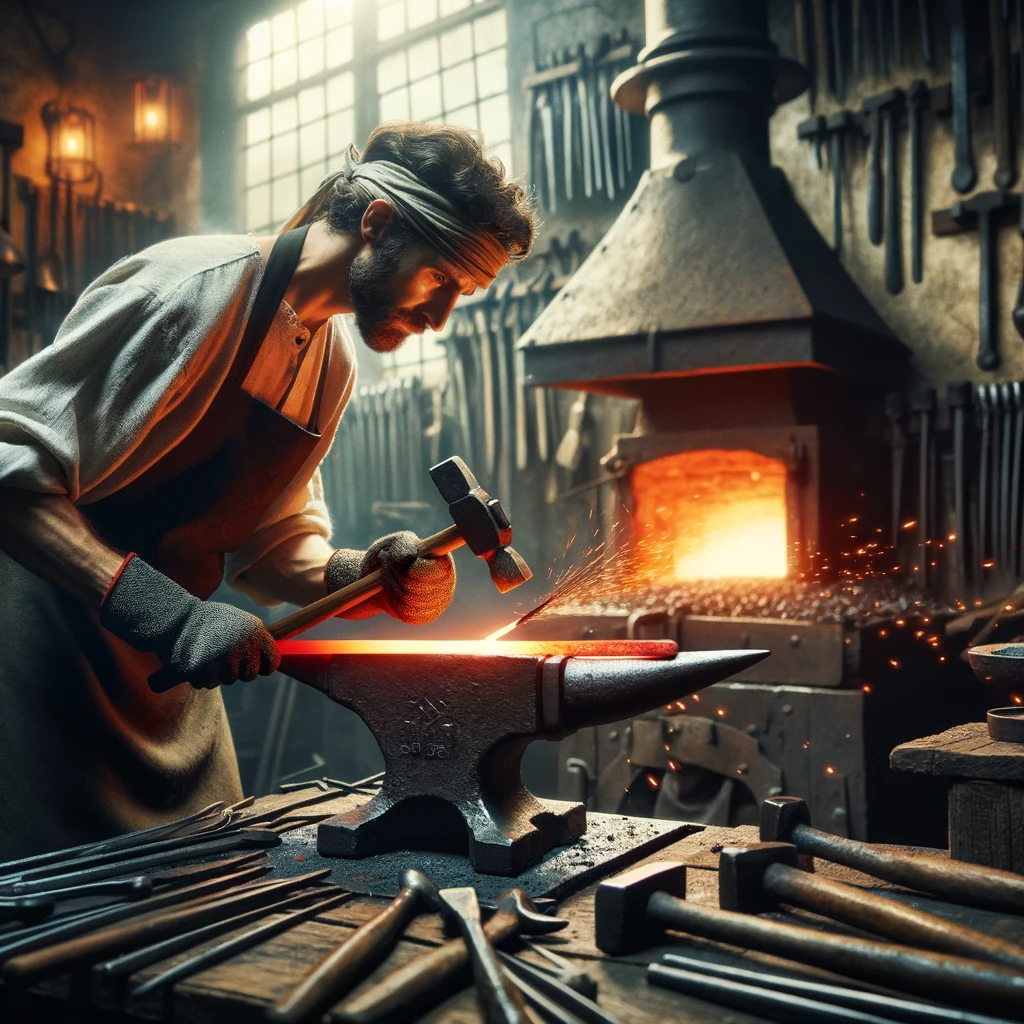
\includegraphics[width=0.5\linewidth]{new_sword.png}
\end{center}
\end{frame}

\begin{frame}
\frametitle{Why a New Programming Language?}
\definecolor{lightblue}{rgb}{0.53, 0.81, 0.98}
\begin{itemize}
	\item new AI ideas are impossible to implement in existing languages
	\item Husky is invented to implementing them with ease
	\item It pushes the boundary of programming towards efficient AGI
\end{itemize}
\begin{center}
\begin{tikzpicture}
    \fill[lightblue] (4.75,0) circle [radius=1.7cm];
    \fill[yellow] (0.5,0) ellipse (2.3cm and 2.0cm);
    \fill[red] (0,0) circle [radius=1.7cm];
     \node[align=center] at (0,0) {Cpp\\ Rust\\ Python\\ Haskell\\ Lean};
     \node[align=center] at (2.25,0) {Husky};
     \node[align=center] at (4.75,0) {Efficient AGI};
\end{tikzpicture}
\end{center}
\end{frame}

\end{document}